\documentclass{beamer}
\usepackage{mathtools}
\usepackage{graphicx}
\usepackage{tikz}
\usepackage[style=alphabetic,maxnames=2,backend=bibtex]{biblatex}
\addbibresource{bibliography.bib}

\graphicspath{{images/}}

\usetheme{Madrid}

\newcommand*{\ex}{\textnormal{ex}}

\title{Double Turán Problem}
\author{Ray Tsai}
\date{\today}

\begin{document}

\frame{\titlepage}

\begin{frame}{Overview}
  \tableofcontents
\end{frame}

\section{Turán Problem}

\begin{frame}
\frametitle{Turán Problem}

\begin{block}{Turán Problem}
  Given a graph $F$, how many edges can an $n$-vertex graph have while containing no copy of $F$ as a subgraph?
\end{block}

\pause

\vspace{0.5cm}

\begin{block}{Turán Number}
  \[
    \ex(n, F) \coloneq \max \{ e(G) : |V(G)| = n \text{ and } F \not\subseteq G \}
  \]
\end{block}
\end{frame}

\begin{frame}
  \frametitle{Turán Problem}

  \begin{block}{Turán's Theorem \cite{Turan1941}}
    For $r + 1 \geq 3$,
    \[
      \ex(n, K_{r + 1}) = e(T_{r}(n)),
    \]
    with equality for graph $G$ only if $G = T_{r}(n)$.
  \end{block}

  \begin{figure}
    \centering
    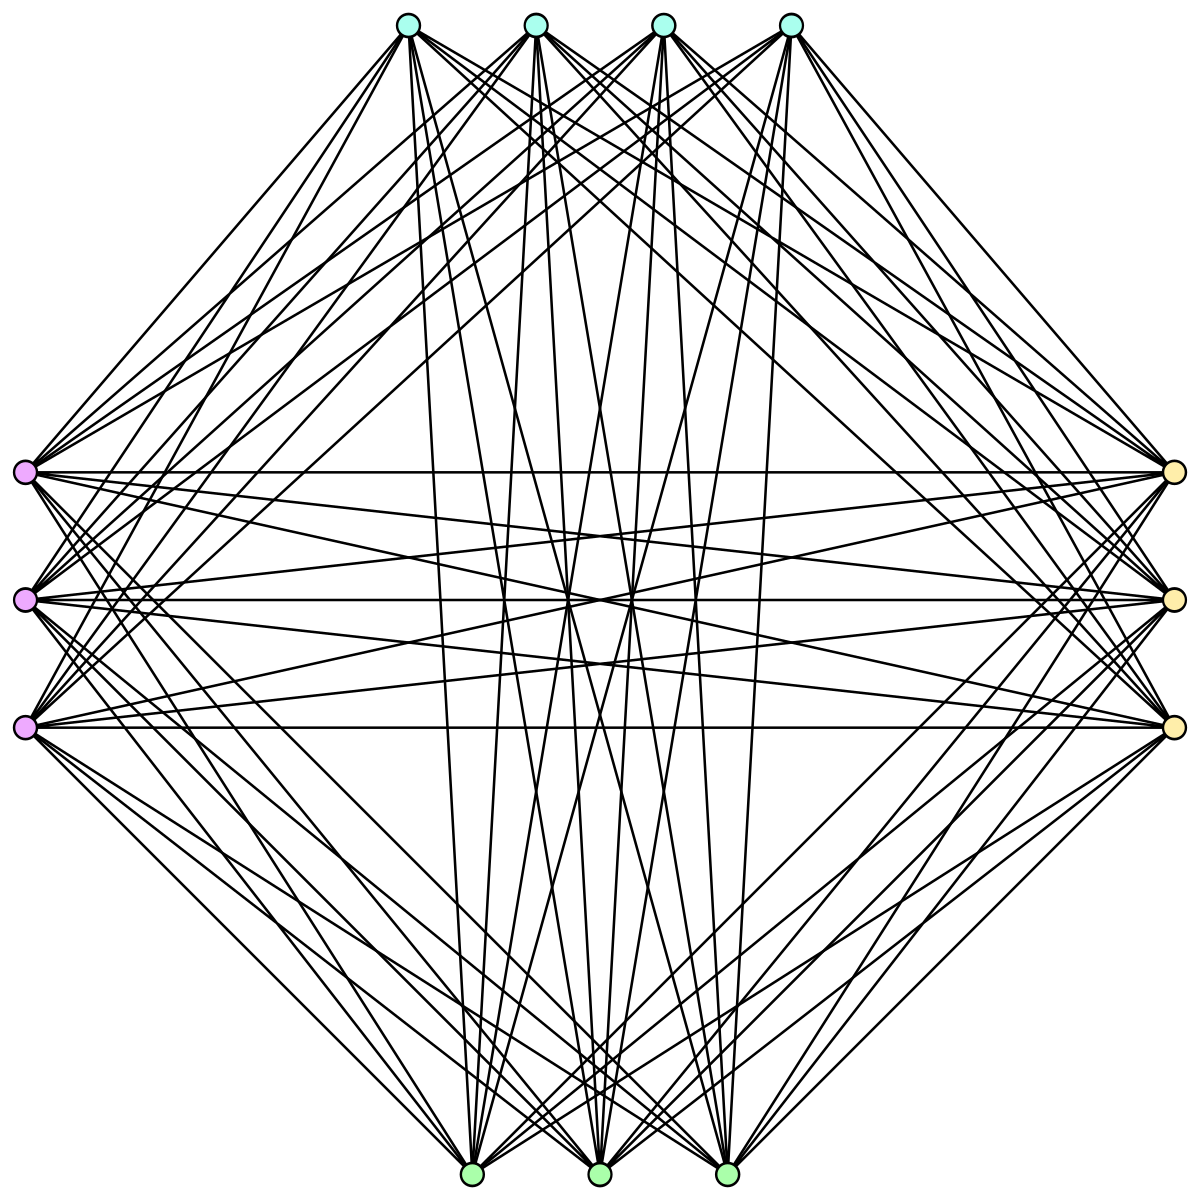
\includegraphics[width=0.3\linewidth]{T_4_13.svg}
    \caption{$T_4(13)$}
  \end{figure}
\end{frame}

\begin{frame}
  \frametitle{Erd\H{o}s-Stone Theorem}

  \begin{block}{Erd\H{o}s-Stone Theorem~\cite{ErdosStone1946}, Simonovits' Theorem~\cite{ErdosSimonovits1966}}
    Let $F$ be any graph of chromatic number $r + 1 \geq 2$. Then $\ex(n, F) = e(T_r(n)) + o(n^2)$ as $n \rightarrow \infty$.
  \end{block}

  \begin{figure}
    \centering
    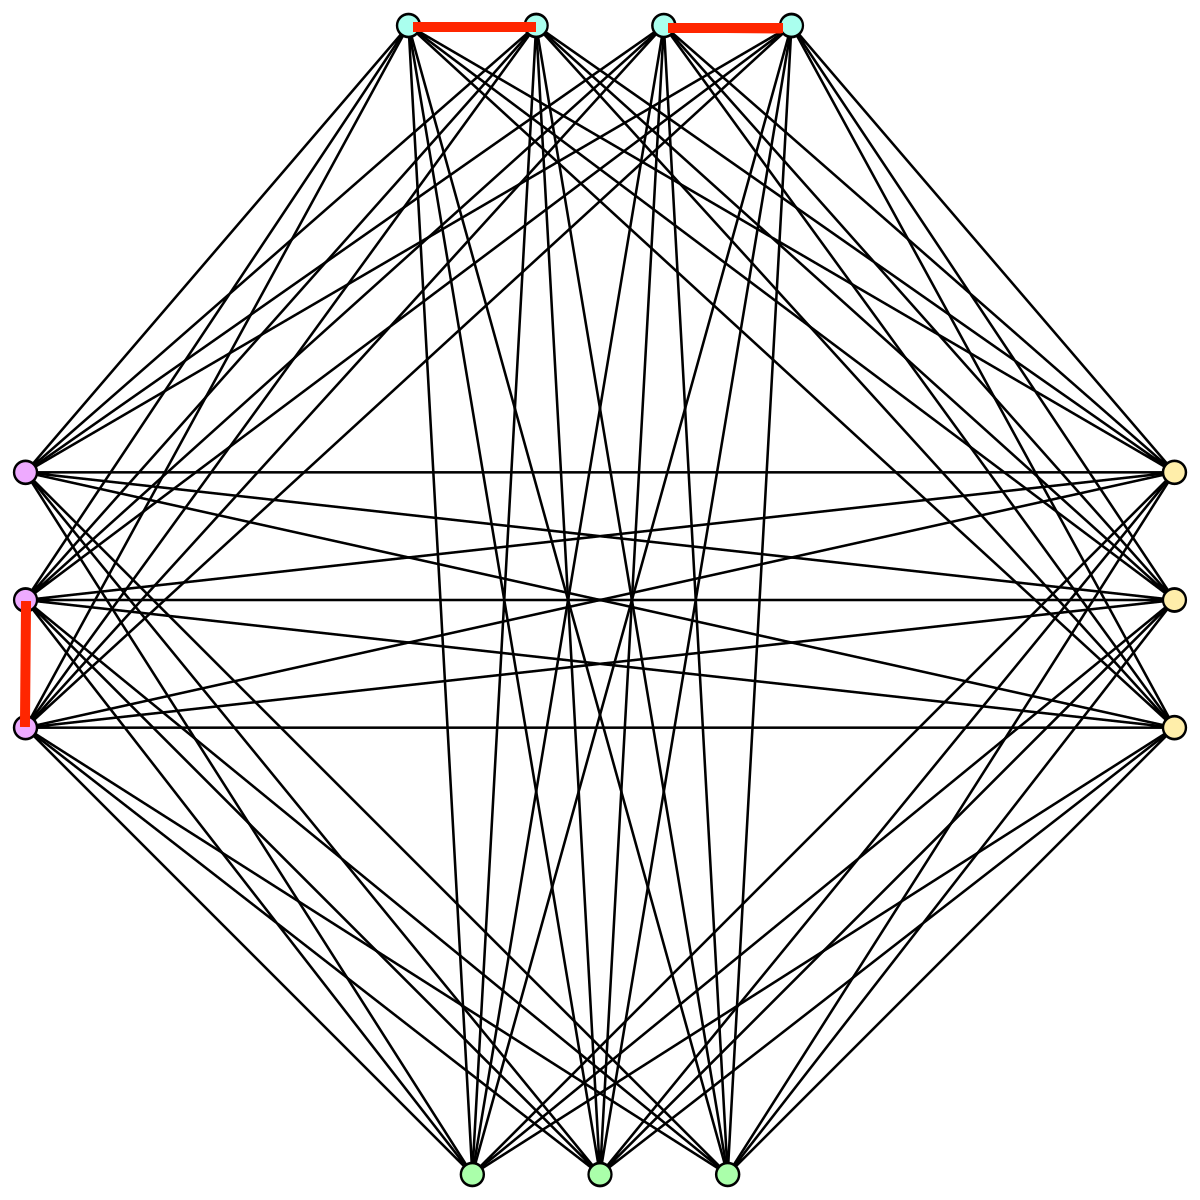
\includegraphics[width=0.25\linewidth]{turan_mod.svg}
  \end{figure}

  \pause

  \begin{block}{Supersaturation Theorem \cite{ErdosSimonovits1983}}
    For all $\epsilon > 0$, there exists $\delta > 0$ such that if $G$ is a $n$-vertex graph with $\ex(n,F) + \epsilon n^2$ edges, then  $G$ contains $\delta n^{v(F)}$ copies of $F$.
  \end{block}
\end{frame}

\section{Double Turán Problem}

\begin{frame}
\frametitle{Double Turán Problem: Definition}

What is the double Turán problem? \pause

\vspace{0.5cm}

Let $G_1, G_2, \ldots, G_m$ be graphs on $[n]$ with $E(F) \not\subseteq E(G_i) \cap E(G_j)$ for distinct $i, j \in [m]$. \pause (\alert{Double $F$-free})

\pause

\begin{block}{Double Turán Problem}
  What is the value of $\phi(m, n, F) = \max \sum_{i = 1}^m G_i$?
\end{block}

\pause

\[
  m\binom{n}{2} \geq \phi(m, n, F) \geq \binom{n}{2} + (m - 1)\ex(n, F)
\]

\pause

Is this tight?
\end{frame}

\begin{frame}
  \frametitle{Double Turán Problem: Main Results}

  \begin{block}{Theorem A}
    Let $n \geq 1$ and $F$ be a non-bipartite graph. Then as $m \to \infty$
    \[ 
      \phi(m, n, F) = (1 + o(1))m \cdot \ex(n, F).
    \]
  \end{block}

  \pause

  \vspace{0.3cm}

  There are $\leq n^{v(F)}$ copies of $F$ over all $G_i$.

  \pause

  \begin{block}{Supersaturation Theorem \cite{ErdosSimonovits1983}}
    For all $\epsilon > 0$, there exists $\delta > 0$ such that if $G$ is a $n$-vertex graph with $\ex(n,F) + \epsilon n^2$ edges, then  $G$ contains $\delta n^{v(F)}$ copies of $F$.
  \end{block}
\end{frame}

\begin{frame}
  \frametitle{Double Turán Problem: Main Results}

  The case for $F = K_r$ can be reduced to a finite computation.

  \pause

  \[
    \phi(3, n, K_3) = \binom{n}{2} + \lfloor n/2\rfloor
  \]

  \pause
  
  But 
  \[
    \lim_{n \to \infty} \frac{\phi(4, n, K_3)}{\binom{n}{2} + 3\lfloor n/4\rfloor} > 1
  \]
\end{frame}

\begin{frame}
  \frametitle{Double Turán Problem: Main Results}

  \begin{figure}
    \centering
    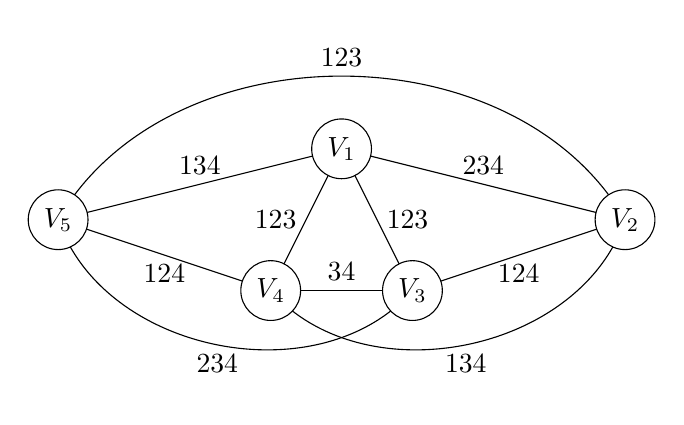
\begin{tikzpicture}[scale=0.9]
    \draw[bend right=60] (4, 0.5) to node[midway, above] {$123$} (-4, 0.5); 
    \draw (-4, 0.5) to node[midway, below] {$124$} (-1, -0.5); 
    \draw (-1, -0.5) to node[midway, above] {$34$} (1, -0.5); 
    \draw (1, -0.5) to node[midway, below] {$124$} (4, 0.5); 
    \draw (0, 1.5) to node[midway, above] {$234$} (4, 0.5); 
    \draw (0, 1.5) to node[midway, above] {$134$} (-4, 0.5); 
    \draw (0, 1.5) to node[midway, left] {$123$} (-1, -0.5); 
    \draw (0, 1.5) to node[midway, right] {$123$} (1, -0.5); 
    \draw[bend left=60] (4, 0.5) to node[midway, below] {$134$} (-1, -0.5); 
    \draw[bend right=60] (-4, 0.5) to node[midway, below] {$234$} (1, -0.5);

    \foreach [count=\i] \x/\y in {0/1.5, 4/0.5, 1/-0.5, -1/-0.5, -4/0.5} { 
      \fill[white] (\x, \y) circle (12pt);
      \draw (\x, \y) circle (12pt);
      \node at (\x, \y) [] {$V_{\i}$}; 
    }
    \end{tikzpicture}
    \caption{Construction for four graphs not containing a double-$K_3$}
  \end{figure}
\end{frame}

\begin{frame}
  \frametitle{Double Turán Problem: Main Results}

  \begin{block}{Theorem B (Wilson)}
    Let $F$ be a graph. If there exists an extremal $F$-free $n$-vertex graph with maximum degree at most $\sqrt{n}/m^2$, then 
    \[ 
      \phi(m, n, F) = \binom{n}{2} + \binom{m}{2}\ex(n,F).
    \]
  \end{block}

  \pause

  By the Erd\H{o}s-Stone theorem, this only applies to certain bipartite graphs.

  \pause

  \vspace{0.5cm}

  e.g. The extremal graph for $P_2$ is a matching, which has maximum degree $1$ and $\ex(n, P_2) = \lfloor n/2 \rfloor$.

  \begin{figure}
    \centering
    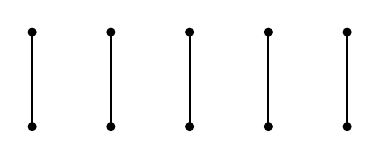
\begin{tikzpicture}[
      vertex/.style = {circle, draw, fill=black, inner sep=1pt},
      edge/.style = {thick}, 
      >=latex  
    ]
    \def\n{5}

  
    \foreach \i in {0,...,\numexpr\n-1\relax}{
      \coordinate (top\i)    at (\i*1, 0); 
      \coordinate (bottom\i) at (\i*1,-1.2);

      \node[vertex] at (top\i)    {};
      \node[vertex] at (bottom\i) {};

      \draw[edge] (top\i) -- (bottom\i);
    }
  \end{tikzpicture}
  \end{figure}  
\end{frame}

\begin{frame}
  \frametitle{Double Turán Problem: Motivation}

  Double Turán problems are closely related to Turán problems for $3$-uniform hypergraphs $H$ through \alert{link graphs}.

  \pause

  \vspace{0.3cm}

  \begin{block}{Link Graph}
    For $i \in V(H)$, define graph $H_i$ with
    \[
      V(H_i) = V(H) \backslash \{i\} \quad \text{and} \quad E(H_i) = \{\{j, k\} : \{i, j, k\} \in E(H)\}.
    \]
  \end{block}
\end{frame}

\begin{frame}
  \frametitle{Double Turán Problem: Motivation}

  Example: Octahedron-free 3-uniform hypergraph $H$

  \only<1>{
    \begin{figure}
      \centering
      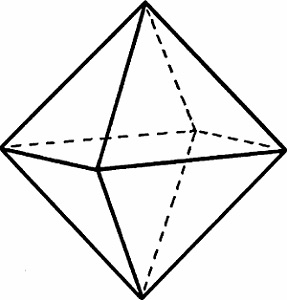
\includegraphics[width=0.15\linewidth]{oct}

      \caption{Octahedron $K_{2,2,2}^{(3)}$}
    \end{figure}
  }

  \only<2>{
    \begin{figure}
      \centering
      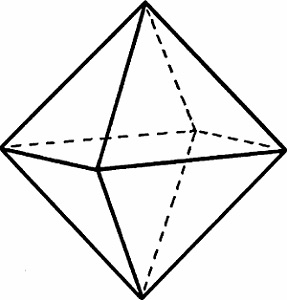
\includegraphics[width=0.15\linewidth]{oct}

      \caption{Octahedron $K_{2,2,2}^{(3)}$}
    \end{figure}

    \begin{block}{Conjecture \cite{Erdos1964}}
      $\ex(n, K_{2,2,2}^{(3)}) = \Theta(n^{11/4})$
    \end{block}
  }

  \only<3>{
    \begin{figure}
      \centering
      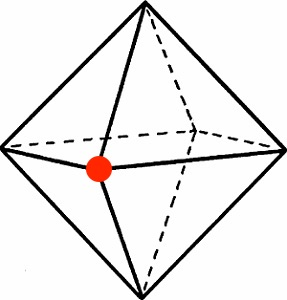
\includegraphics[width=0.15\linewidth]{oct_linked1}

      \caption{Octahedron $K_{2,2,2}^{(3)}$}
    \end{figure}

    \begin{block}{Conjecture \cite{Erdos1964}}
      $\ex(n, K_{2,2,2}^{(3)}) = \Theta(n^{11/4})$
    \end{block}
  }

  \only<4>{
    \begin{figure}
      \centering
      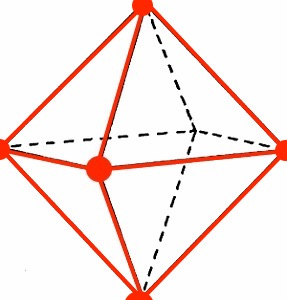
\includegraphics[width=0.15\linewidth]{oct_linked2}

      \caption{Octahedron $K_{2,2,2}^{(3)}$}
    \end{figure}

    \begin{block}{Conjecture \cite{Erdos1964}}
      $\ex(n, K_{2,2,2}^{(3)}) = \Theta(n^{11/4})$
    \end{block}
  }

  \only<5>{
    \begin{figure}
      \centering
      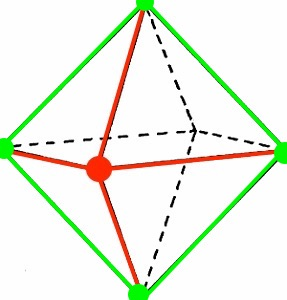
\includegraphics[width=0.15\linewidth]{oct_linked3}

      \caption{Octahedron $K_{2,2,2}^{(3)}$}
    \end{figure}

    \begin{block}{Conjecture \cite{Erdos1964}}
      $\ex(n, K_{2,2,2}^{(3)}) = \Theta(n^{11/4})$
    \end{block}
  }

  \only<6>{

    \begin{figure}
      \centering
      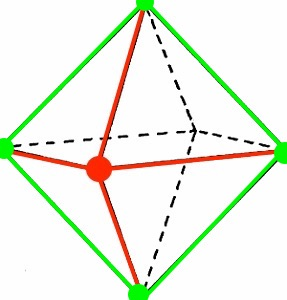
\includegraphics[width=0.15\linewidth]{oct_linked3}
      
      \caption{Octahedron $K_{2,2,2}^{(3)}$}
    \end{figure}

    \begin{block}{Conjecture \cite{Erdos1964}}
      $\ex(n, K_{2,2,2}^{(3)}) = \Theta(n^{11/4})$
    \end{block}

    \vspace{0.1cm}

    \begin{center}
      $H$ is octahedron-free $\implies$ $H_1, H_2, \ldots, H_n$ are double $K_{2,2}$-free.
    \end{center}
  
    \[
      \boxed{\ex(n, K_{2,2,2}^{(3)}) \leq \phi(n, n, K_{2,2})}
    \]
  }

  \only<7>{
    \begin{figure}
      \centering
      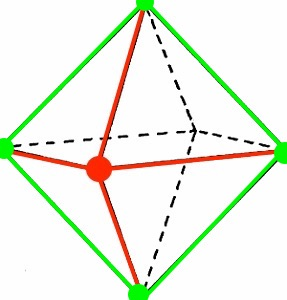
\includegraphics[width=0.15\linewidth]{oct_linked3}
      
      \caption{Octahedron $K_{2,2,2}^{(3)}$}
    \end{figure}

    \begin{block}{Conjecture \cite{Erdos1964}}
      $\ex(n, K_{2,2,2}^{(3)}) = \Theta(n^{11/4})$
    \end{block}

    \vspace{0.1cm}

    \begin{center}
      $H$ is octahedron-free $\implies$ $H_1, H_2, \ldots, H_n$ are double $K_{2,2}$-free.
    \end{center}
  
    \[
      \boxed{\ex(n, K_{2,2,2}^{(3)}) = \Theta(\phi(n, n, K_{2,2}))}
    \]
  }
\end{frame}

\section{Induced Double Turán Problem}

\begin{frame}
  \frametitle{Induced Double Turán Problem: Definition}

  What is the \alert{induced} double Turán problem? \pause

  \begin{block}{Induced Graphs}
    We call graphs $G_1, G_2, \ldots, G_m$ \alert{induced} if each $G_i$ is an induced subgraph of $\bigcup_{i = 1}^m G_i$.
  \end{block}

  \pause

  In other words, if $\{u, v\} \in E(G_i)$ and $u, v \in V(G_j)$, then $\{u, v\} \in E(G_j)$.

  \pause

  \vspace{0.5cm}

  Let graphs $G_1, G_2, \ldots, G_m$ be induced and double $F$-free.

  \begin{block}{Induced Double Turán Problem}
    What is the value of $\phi^*(m, n, F) = \max \sum_{i = 1}^m e(G_i)$?
  \end{block}

  \pause

  \[
    \phi(m, n, F) \geq \phi^*(m, n, F)
  \]
\end{frame}

\begin{frame}

  \frametitle{Induced Double Turán Problem: Conjecture}

  \begin{block}{Induced Double Turán Problem}
    What is the value of $\phi^*(m, n, F) = \max \sum_{i = 1}^m e(G_i)$?
  \end{block}

  \[
    \phi^*(m, n, F) \geq \max\Bigl\{\binom{n}{2} + \binom{v(F) - 1}{2}(m - 1), \, m \cdot \ex(n,F)\Bigr\}.
  \]

  \pause

  Is it tight?

  \pause

  \begin{block}{Conjecture}
    Let $F$ be any non-empty graph and $m, n \geq 1$. Then
    \[ 
      \phi^*(m,n,F) = \Theta(m \cdot \ex(n,F) + n^2).
    \]
  \end{block}
\end{frame}

\begin{frame}
  \frametitle{Induced Double Turán Problem: Main Results}


  \begin{block}{Theorem C}
    For $m \geq 3$ and non-bipartite $F$, if $n$ is large enough, then
    \[
      \phi^*(m, n, F) = m \cdot \ex(n, F),
    \]
    with equality only for identical extremal $n$-vertex $F$-free graphs.
  \end{block}

  \pause

  $\implies$ Conjecture is true for non-bipartite $F$.

  \pause

  \vspace{0.5cm}

  For $F = K_r$, this theorem applies for all $n$.
\end{frame}

\begin{frame}
  \frametitle{Induced Double Turán Problem: Motivation}

  \begin{block}{Generalized Turán problem}
    What is the maximum number $\ex(n, F, K_3)$ of triangles in an $n$-vertex $F$-free graph $G$?
  \end{block}

  Studied by Alon and Shikhelman \cite{AlonShikhelman2016} and Kostochka, Mubayi and Verstraete \cite{KostochkaMubayiV2015,MubayiMukherjee2023,MubayiV2016}.

  \pause 

  \vspace{0.7cm}

  For $i \in V(G)$, define $G_i$ with
  \[
    V(G_i) = V(G) \quad \text{and} \quad E(G_i) = \{\{j, k\} : \{i, j\}, \{j, k\}, \{i, k\} \in E(G)\}
  \]
\end{frame}

\begin{frame}
  \frametitle{Induced Double Turán Problem: Motivation}

  Ex. Octahedron-free graph $G$.

  \only<1>{
    \begin{figure}
      \begin{minipage}{0.48\textwidth}
        \centering
        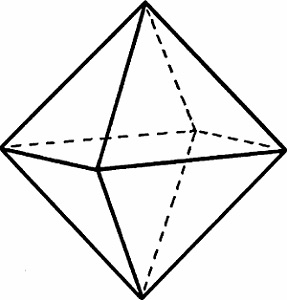
\includegraphics[width=0.45\linewidth]{oct}
        \caption{Octahedron}
      \end{minipage}
      \hfill
      \begin{minipage}{0.48\textwidth}
        \centering
        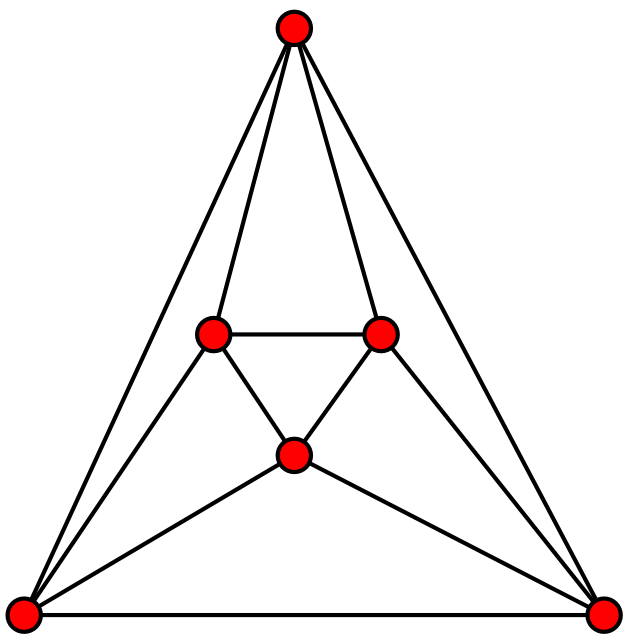
\includegraphics[width=0.45\linewidth]{K222}
        \caption{Octahedron Graph $K_{2,2,2}$}
      \end{minipage}
    \end{figure}
  }

  \only<2>{
    \begin{figure}
      \begin{minipage}{0.48\textwidth}
        \centering
        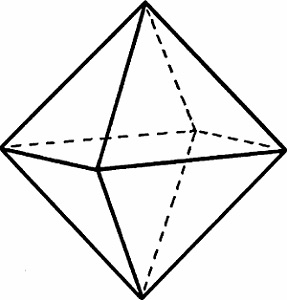
\includegraphics[width=0.45\linewidth]{oct}
        \caption{Octahedron}
      \end{minipage}
      \hfill
      \begin{minipage}{0.48\textwidth}
        \centering
        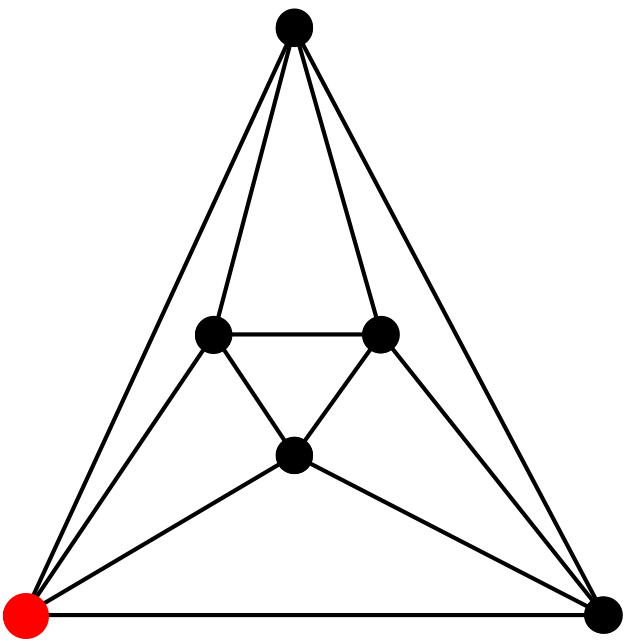
\includegraphics[width=0.45\linewidth]{K222_linked0}
        \caption{Octahedron Graph $K_{2,2,2}$}
      \end{minipage}
    \end{figure}
  }

  \only<3>{
    \begin{figure}
      \begin{minipage}{0.48\textwidth}
        \centering
        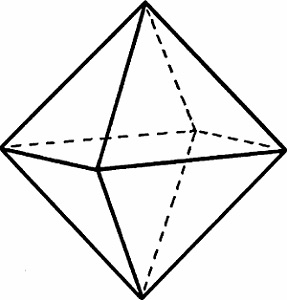
\includegraphics[width=0.45\linewidth]{oct}
        \caption{Octahedron}
      \end{minipage}
      \hfill
      \begin{minipage}{0.48\textwidth}
        \centering
        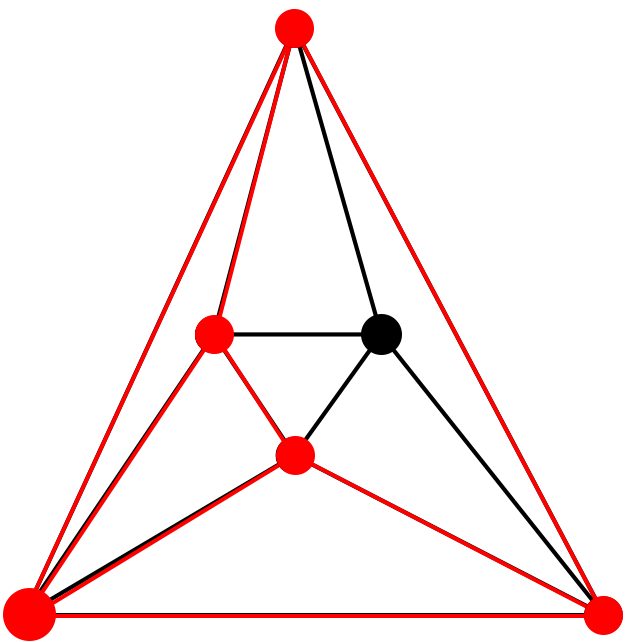
\includegraphics[width=0.45\linewidth]{K222_linked1}
        \caption{Octahedron Graph $K_{2,2,2}$}
      \end{minipage}
    \end{figure}
  }

  \only<4>{
    \begin{figure}
      \begin{minipage}{0.48\textwidth}
        \centering
        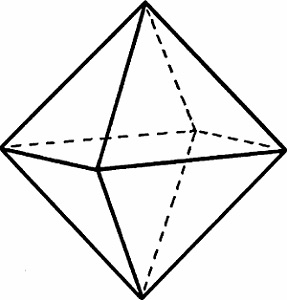
\includegraphics[width=0.45\linewidth]{oct}
        \caption{Octahedron}
      \end{minipage}
      \hfill
      \begin{minipage}{0.48\textwidth}
        \centering
        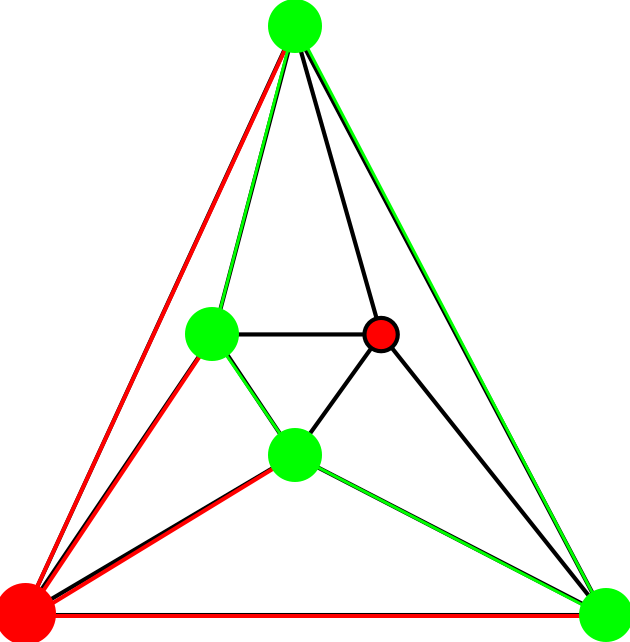
\includegraphics[width=0.45\linewidth]{K222_linked2}
        \caption{Octahedron Graph $K_{2,2,2}$}
      \end{minipage}
    \end{figure}
  }

  \only<5>{
    \begin{figure}
      \begin{minipage}{0.48\textwidth}
        \centering
        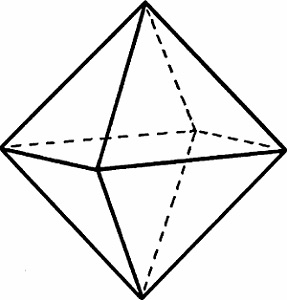
\includegraphics[width=0.45\linewidth]{oct}
        \caption{Octahedron}
      \end{minipage}
      \hfill
      \begin{minipage}{0.48\textwidth}
        \centering
        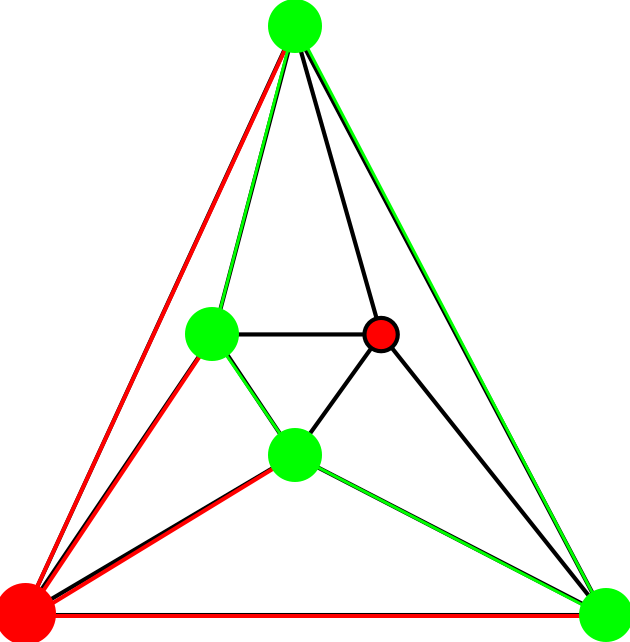
\includegraphics[width=0.45\linewidth]{K222_linked2}
        \caption{Octahedron Graph $K_{2,2,2}$}
      \end{minipage}
    \end{figure}
  
    \vspace{0.1cm}
  
    \begin{center}
      $G$ is $K_{2,2,2}$-free $\implies$ $G_1, G_2, \ldots, G_n$ are induced and double $K_{2, 2}$-free.
    \end{center}
  
    \[
      \boxed{\ex(n, K_{2,2,2}, K_3) \leq \phi^*(n, n, K_{2,2})}
    \]
  }

  \only<6>{
    \begin{figure}
      \begin{minipage}{0.48\textwidth}
        \centering
        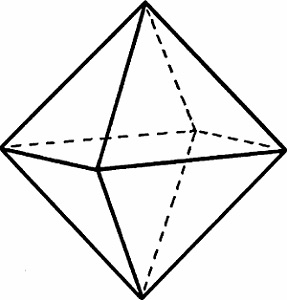
\includegraphics[width=0.45\linewidth]{oct}
        \caption{Octahedron}
      \end{minipage}
      \hfill
      \begin{minipage}{0.48\textwidth}
        \centering
        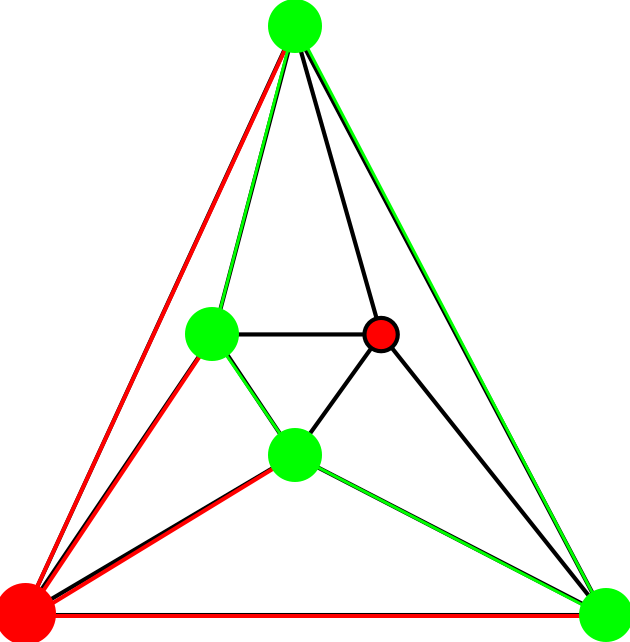
\includegraphics[width=0.45\linewidth]{K222_linked2}
        \caption{Octahedron Graph $K_{2,2,2}$}
      \end{minipage}
    \end{figure}
  
    \vspace{0.1cm}
  
    \begin{center}
      $G$ is $K_{2,2,2}$-free $\implies$ $G_1, G_2, \ldots, G_n$ are induced and double $K_{2, 2}$-free.
    \end{center}
  
    \[
      \boxed{\ex(n, K_{2,2,2}, K_3) = \Theta(\phi^*(n, n, K_{2,2}))}
    \]
  }
\end{frame}

\begin{frame}
  \frametitle{Induced Double Turán Problem: Motivation}

  \begin{block}{Conjecture}
    Let $F$ be any non-empty graph and $m, n \geq 1$. Then
    \[ 
      \phi^*(m, n, F) = \Theta(m \cdot \ex(n, F) + n^2).
    \]
  \end{block}

  \vspace{0.3cm}

  Conjecture implies
  \[
    \ex(n, K_{2, 2, 2}, K_3) = \Theta(\phi^*(n, n, K_{2, 2})) = \Theta(n^{5/2}).
  \]
\end{frame}

\begin{frame}
  \frametitle{Main Results}

  \begin{block}{Theorem D}
    Let $P$ be a path with two edges. Then $\phi(n, n, P) = \Omega(n^{5/2})$, whereas $\phi^*(n, n, P) = o(n^{5/2})$, as $n \rightarrow \infty$. In particular, 
    \[ 
      \lim_{n \rightarrow \infty} \frac{\phi^*(n, n, P)}{\phi(n, n, P)} = 0.
    \]
  \end{block}

  \pause

  \vspace{0.3cm}

  This shows that $\phi(m, n, F)$ and $\phi^*(m, n, F)$ can be very different problems.
\end{frame}

\section{Proof of Theorem B}

\begin{frame}
  \frametitle{Proof of Theorem B: Upper Bound}

  \begin{block}{Theorem B (Wilson)}
    Let $F$ be a graph. If there exists an extremal $F$-free $n$-vertex graph with maximum degree at most $\sqrt{n}/m^2$, then 
    \[ 
      \phi(m, n, F) = \binom{n}{2} + \binom{m}{2}\ex(n,F).
    \]
  \end{block}

  \pause

  We need to show
  \[  
    \phi(m, n ,F) \leq \binom{n}{2} + \ex(n, F)\binom{m}{2}.  
  \]

  \pause
  
  Let $E_S$ be the set of edges in exactly $\{G_i\}_{i \in S}$.

  \pause

  \[
    \implies \sum_{i = 1}^m e(G_i) = \sum_{S \subseteq [m]} |S||E_S| \leq \binom{n}{2} + \sum_{S \subseteq [m], |S| \geq 2} (|S| - 1)|E_S|.
  \]
\end{frame}

\begin{frame}

  \frametitle{Proof of Theorem B: Upper Bound}

  \[
    \sum_{\substack{S \subseteq [m] \\ |S| \geq 2}} (|S| - 1)|E_S| = \sum_{\substack{S \subseteq [m], \\ |S| = 2}} \sum_{T \supseteq S} \frac{(|T| - 1)|E_T|}{\binom{|T|}{2}} \leq \sum_{\substack{S \subseteq [m], \\ |S| = 2}} \sum_{T \supseteq S} |E_T|,
  \]
  as each $T \in [m]$ with $|T| \geq 2$ is counted $\binom{|T|}{2}$ times.
\end{frame}

\begin{frame}
  \frametitle{Proof of Theorem B: Upper Bound}

  Observation: If $|S| \geq 2$, the edge set $\bigcup_{T \supseteq S} E_T$ is $F$-free.

  \pause

  \vspace{0.3cm}

  \[
    \left|\bigcup_{T \supseteq S} E_T\right| = \sum_{T \supseteq S} |E_T| \leq \ex(n, F)
  \]
  \pause

  \vspace{0.3cm}

  \[
    \implies \sum_{\substack{S \subseteq [m] \\ |S| \geq 2}} (|S| - 1)|E_S| \leq \sum_{\substack{S \subseteq [m], \\ |S| = 2}} \sum_{T \supseteq S} |E_T| \leq \binom{m}{2}\ex(n, F)
  \]
  This proves the upper bound.
\end{frame}

\begin{frame}
  \frametitle{Proof of Theorem B: Lower Bound}

  We need to show
  \[  
    \phi(m, n ,F) \geq \binom{n}{2} + \ex(n, F)\binom{m}{2}.  
  \]

  \pause
  \vspace{0.3cm}

  For $1 \leq i < j \leq m$, let $H_{ij}$ be an extremal $F$-free graph on $[n]$ with maximum degree $\Delta(H_{ij}) \leq \sqrt{n}/m^2$

  \pause

  \vspace{0.5cm}

  $\implies$ We can pack these $\binom{m}{2}$ $H_{ij}$'s into $[n]$ s.t. $E(H_{i_1j_1}) \cap E(H_{i_2j_2}) = \emptyset$
\end{frame}

\begin{frame}
  \frametitle{Proof of Theorem B: Lower Bound}

  For $i \in [m]$, put 
  \[
    G_i = H_{1i} \cup H_{2i} \cup \cdots \cup H_{im}
  \]
  \pause

  Then $G_i \cap G_j = H_{ij} \implies F\text{-free}$

  \pause

  \vspace{0.7cm}

  Add edges not in any of $H_{ij}$ to $G_1$.
  \[
    \sum_{i = 1}^m e(G_i) = 2\underbrace{\sum e(H_{ij})}_{\binom{m}{2}\ex(n, F)} + \underbrace{\left|E(K_n)\backslash \bigsqcup E(H_{ij})\right|}_{\binom{n}{2} - \binom{m}{2}\ex(n, F)} = \binom{n}{2} + \binom{m}{2}\ex(n, F)
  \]
\end{frame}

\section{Proof of Theorem C}

\begin{frame}
  \frametitle{Proof of Theorem C: Complete Graph Case}

  \begin{block}{Theorem C: Complete Graph Case}
    Let $m, n, r \geq 3$. Then 
    \[
      \phi^*(m, n, K_{r}) = m \cdot e(T_{r - 1}(n)),
    \]
    with equality for induced $K_{r}$-free graphs $G_1, G_2, \dots, G_m$ only if $G_1 = G_2 = \dots = G_m = T_{r - 1}(n)$. 
  \end{block}

  \pause

  \vspace{0.7cm}

  IDEA: Reduce to $m = 2$.
\end{frame}

\begin{frame}
  \frametitle{Proof of Theorem C: Complete Graph Case}

  \begin{center}
    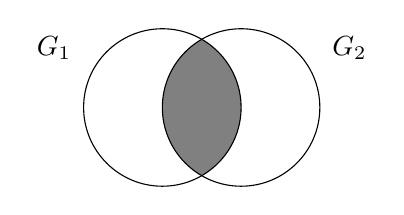
\begin{tikzpicture}
      % ---- fill only the intersection -----------------
      \begin{scope}
        \clip (0,0) circle (1);          % keep area inside left circle
        \fill[gray] (1,0) circle (1);    % paint overlap with right circle
      \end{scope}
    
      % ---- circle outlines ----------------------------
      \draw (0,0) circle (1);
      \draw (1,0) circle (1);
    
      % ---- labels outside the circles -----------------
      \node[left=1pt]  at (-1,0.75) {$G_1$};
      \node[right=1pt] at (2,0.75) {$G_2$};
    \end{tikzpicture}
  \end{center}

  \pause

  $G_1 \cap G_2$ (gray area) is double $K_r$-free.

  \pause

  \vspace{0.5cm}

  If $G_1, G_2$ intersects in $t$ vertices, then
  \[
    e(G_1) + e(G_2) \leq \binom{n - t}{2} + (n - t)t + 2T_{r - 1}(t)
  \]

  \pause

  $\implies$ we are done if the unique maximum occurs at $t = n$.
\end{frame}

\begin{frame}
  \frametitle{Proof of Theorem C: Complete Graph Case}
  \begin{figure}
    \begin{minipage}{0.4\textwidth}
      \centering
        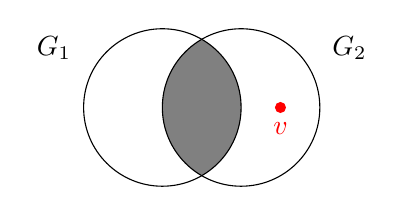
\begin{tikzpicture}
        % ---- fill only the intersection -----------------
        \begin{scope}
          \clip (0,0) circle (1);          % keep area inside left circle
          \fill[gray] (1,0) circle (1);    % paint overlap with right circle
        \end{scope}
          
        % ---- circle outlines ----------------------------
        \draw (0,0) circle (1);
        \draw (1,0) circle (1);
          
        % ---- labels outside the circles -----------------
        \node[left=1pt]  at (-1,0.75) {$G_1$};
        \node[right=1pt] at (2,0.75) {$G_2$};
        \fill[red] (1.5,0) circle (2pt) node[below=2pt] {$v$};
    \end{tikzpicture}
    \end{minipage}
    \begin{minipage}{0.05\textwidth}
      \centering
      $>$
    \end{minipage}
    \begin{minipage}{0.4\textwidth}
      \centering
        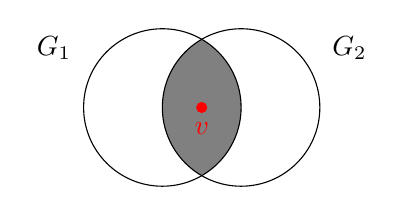
\begin{tikzpicture}
        % ---- fill only the intersection -----------------
        \begin{scope}
          \clip (0,0) circle (1);          % keep area inside left circle
          \fill[gray] (1,0) circle (1);    % paint overlap with right circle
        \end{scope}
          
        % ---- circle outlines ----------------------------
        \draw (0,0) circle (1);
        \draw (1,0) circle (1);
          
        % ---- labels outside the circles -----------------
        \node[left=1pt]  at (-1,0.75) {$G_1$};
        \node[right=1pt] at (2,0.75) {$G_2$};
        \fill[red] (0.5,0) circle (2pt) node[below=2pt] {$v$};
    \end{tikzpicture}
    \end{minipage}
  \end{figure}

  \pause

  Put $f(t, r) \coloneq \binom{n - t}{2} + (n - t)t + 2T_{r - 1}(t)$

  \vspace{0.5cm}

  For example, if $r = 4$,
  \[
    f(t + 1, 4) - f(t, 4) = -t + 1 + 2[\underbrace{T_3(t + 1) - T_3(t)}_{t - \left\lceil\frac{t}{2}\right\rceil}] = t + 1 - 2\left\lceil\frac{t}{2}\right\rceil > 0
  \]

  \pause

  $\implies$ The larger the intersection, the larger the sum of edges.

  \pause

  \vspace{0.3cm}

  $\implies$ The best we can do is $G_1 = G_2 = T_3(n)$.
\end{frame}

\section{Concluding Remarks}

\begin{frame}
  \frametitle{Concluding Remarks: Induced Double Turán Problem}

  \begin{block}{Conjecture}
    Let $F$ be any non-empty graph and $m, n \geq 1$. Then
    \[ 
      \phi^*(m,n,F) = \Theta(m \cdot \ex(n,F) + n^2).
    \]
  \end{block}

  \pause

  \vspace{0.3cm}

  This conjecture is broadly open for bipartite graphs.

  \vspace{0.2cm}

  \begin{center}

  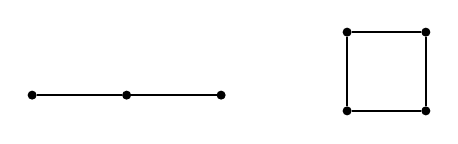
\begin{tikzpicture}[
    vertex/.style = {circle, draw, fill=black, inner sep=1pt},
    edge/.style   = {thick}
  ]

    %% ---- Path P3 (length 2) ----
    \node[vertex] (p1) at (0,0)   {};
    \node[vertex] (p2) at (1.2,0) {};
    \node[vertex] (p3) at (2.4,0) {};

    \draw[edge] (p1) -- (p2) -- (p3);

    %% ---- 4‑cycle C4, shifted to the right ----
    \begin{scope}[shift={(4,0)}] % change (4,0) to move closer/farther
      \node[vertex] (c1) at (0, 0.8) {};
      \node[vertex] (c2) at (1, 0.8) {};
      \node[vertex] (c3) at (1,-0.2) {};
      \node[vertex] (c4) at (0,-0.2) {};

      \draw[edge] (c1) -- (c2) -- (c3) -- (c4) -- (c1);
    \end{scope}
  \end{tikzpicture}

  \end{center}

  \pause

  Solving the conjecture would give a solution to $\ex(n, K_{2,2,2}, K_3)$.
\end{frame}

\begin{frame}
  \frametitle{Concluding Remarks: Double Turán Problem}

  For non-bipartite $F$, $\phi(m, n, F)$ case is likely intractable.

  \pause

  \vspace{0.5cm}

  We only know $\phi(3, n, K_3) = \binom{n}{2} + \lfloor n/2\rfloor$. The rest is open.

  \pause

  \vspace{0.2cm}

  \[
    \lim_{n \to \infty} \frac{\phi(4, n, K_3)}{m\binom{n}{2}} = ??
  \]
\end{frame}

\begin{frame}[allowframebreaks] 
  \frametitle{References}
  \printbibliography
\end{frame}
\end{document}
